\documentclass{article}

% if you need to pass options to natbib, use, e.g.:
% \PassOptionsToPackage{numbers, compress}{natbib}
% before loading nips_2016
%
% to avoid loading the natbib package, add option nonatbib
% \usepackage[nonatbib]{nips_2016}

\usepackage{nips_2016}

% to compile a camera-ready version, add the [final] option, e.g.:
% \usepackage[final]{nips_2016}

\usepackage[utf8]{inputenc} % allow utf-8 input
\usepackage[T1]{fontenc}    % use 8-bit T1 fonts
\usepackage{hyperref}       % hyperlinks
\usepackage{url}            % simple URL typesetting
\usepackage{booktabs}       % professional-quality tables
\usepackage{amsfonts}       % blackboard math symbols
\usepackage{nicefrac}       % compact symbols for 1/2, etc.
\usepackage{microtype}      % microtypography
\usepackage{graphicx}       %PICTSCHA
\usepackage{amsmath}        %METH, ok appears to be included in the amsfontz





%%%%%%%%%%
% citation stuff
%%%%%%%%

\usepackage{natbib} 
%bibstyle muss einer da sein, 
% setimmt wie der kram an \cite aussieht.
% https://de.wikibooks.org/wiki/LaTeX-W%C3%B6rterbuch:_bibliographystyle
%https://de.sharelatex.com/learn/Bibtex_bibliography_styles
%\bibliographystyle{abbrvnat} 
\bibliographystyle{unsrt} 
%\bibliographystyle{plainnat}









\title{Superawesome Graph Generation}

% The \author macro works with any number of authors. There are two
% commands used to separate the names and addresses of multiple
% authors: \And and \AND.
%
% Using \And between authors leaves it to LaTeX to determine where to
% break the lines. Using \AND forces a line break at that point. So,
% if LaTeX puts 3 of 4 authors names on the first line, and the last
% on the second line, try using \AND instead of \And before the third
% author name.

\author{
  Stefan Mautner\\
  Department of Computer Science\\
  Albert-Ludwigs University Freiburg\\
  Freiburg, 79085  \\
  \texttt{mautner@cs.uni-freiburg.de} \\
  %% examples of more authors
  %% \And
  %% Coauthor \\
  %% Affiliation \\
  %% Address \\
  %% \texttt{email} \\
  %% \AND
  %% Coauthor \\
  %% Affiliation \\
  %% Address \\
  %% \texttt{email} \\
  %% \And
  %% Coauthor \\
  %% Affiliation \\
  %% Address \\
  %% \texttt{email} \\
  %% \And
  %% Coauthor \\
  %% Affiliation \\
  %% Address \\
  %% \texttt{email} \\
}

\begin{document}
% \nipsfinalcopy is no longer used

\maketitle

\begin{abstract}
    \cite{rfam}Nulla pulvinar ante rutrum efficitur pellentesque. Donec augue tortor, dapibus vitae quam at, ultricies bibendum mauris. Etiam est nisi, ultricies vitae est euismod, rutrum eleifend ligula. Donec dictum orci ullamcorper ipsum vulputate gravida. Phasellus dignissim commodo feugiat. Proin bibendum interdum malesuada. Phasellus nibh dolor, pulvinar vel hendrerit vitae, egestas eu mi. Aenean ornare mauris purus, porta euismod turpis tristique eget. Maecenas magna velit, tempus aliquet nunc quis, vulputate faucibus dui. Cras egestas viverra libero faucibus vehicula. Donec molestie lectus in mattis convallis.
\end{abstract}
\section{Introduction}


% 
\begin{figure}[ht]
      \centering
        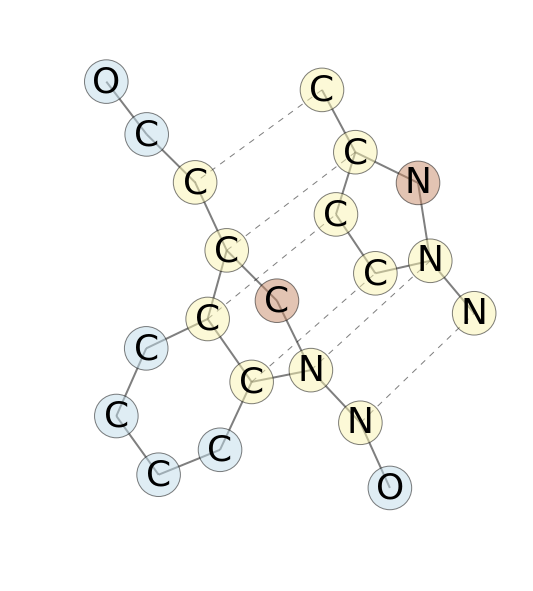
\includegraphics[width=0.2\linewidth]{images/cip.png}
      \caption{Sample figure caption.}
      \label{nazis}
\end{figure}

Lorem ipsum dolor sit amet, consectetur adipiscing elit. Nullam tempus nunc tempus, pretium leo sed, blandit ante. Nulla sit amet consectetur nunc. Curabitur dictum, risus in eleifend tincidunt, ipsum libero dapibus magna, eu lacinia purus ligula ut lorem. Sed vel eleifend massa, eget tincidunt erat. Nulla vel semper ipsum, quis tincidunt dolor. Duis convallis diam at auctor laoreet. Maecenas at lorem egestas, mollis felis sit amet, sagittis est. Sed eget lorem ut sapien porttitor malesuada. Fusce vehicula, nunc sit amet auctor ultrices, odio ligula gravida enim, sed bibendum risus quam sit amet justo. Donec eget mauris at tortor iaculis finibus. Suspendisse sollicitudin tellus quam, eget aliquam ipsum mollis vitae. Morbi et hendrerit eros, ut consequat justo. Ut blandit lobortis sem. Donec sem felis, scelerisque tincidunt nibh sit amet, eleifend consectetur magna. Nunc ultricies gravida commodo. Morbi vestibulum tellus nec turpis imperdiet tempor

\section{Method}
Previously Costa \cite{costa14} introduced a method
on the construction of novel graphs according to a distribution given by
example graphs. Graphs were vectorized via a \emph{decomposition kernel}
to train a machine learning model, e.g. an SVM.
Fragments of the graphs would be collected in 
a \emph{grammar} (resembling a string grammar) to alter the 
set of graphs incrementally. Changes to a graph are evaluated with the model. 
We present a method to increase the flexibility of the graph grammar.


%%%%%%%%%%%%%%%%%%%%%%%%%%%%%%%%%%%%%%%%%%%%%%%%%%%%CONTINUE THE WRITING HERE! 
\textbf{Modification to the grammar.}
We work with different CIPs that consider a contracted version
of the original graphs. We obtain a contracted graph $G'$ by contracting edges
in $G$. After a contraction, the set of contracted vertices of the 
created vertex is accessible with the $contracted$ function.
We extract $C_{R}^v(G')$ and $I_{R,T}^v(G')$ as usual, but from $G'$. 
The core graph $C_{R}^v(G',G)$ is induced by the nodes 
$\bigcup\limits_{u \in C_R^v(G')} contracted(u)$.
The new interface graph $I_{R,B}^v(G',G)$ is then obtained by the nodes 
$\{ w | d(w,v) \leq B \wedge v\in C_R^v(G',G) \wedge w \in G \wedge w 
\notin C_R^v(G',G) \}$.  $B$ is the thickness of the base graph. 
At this point we can construct a CIP from $C_R^v(G',G)$ and $I_{R,B}^v(G',G)$. 
To find a congruent CIP, we previously only compared the hashed $I_{R,T}^v(G)$ 
graphs. By hashing the hashes of $I_{R,T}^v(G')$ and $I_{R,B}^v(G,G')$ we 
increase the specificity of this comparison. The vertices in $I_{R,B}^v(G,G')$ 
might have been relabeled to represent a concept of its $contracted$ set. In 
our test, we will contract according to the 
secondary RNA structure and label the resulting vertex accordingly e.g.
'Hairpin loop'. This way we encode far reaching and abstract 
information about the surrounding vertices in our CIP interface matching.



% graph contration, interface trick
% change to congruency
\textbf{An improvement to the notion of congruency.}
For CIPs to be congruent, isomorphism is required. 
We expand this requirement to incorporate
the distance to nodes in the core graph when determining if graphs are 
congruent.
$\forall u \in I_{R,T}^v(G) : 
\underset{z \in  C_{R}^v(G)}{\min} d(u,z) = 
\underset{z' \in  C_{R}^{v'}(G')}{\min} d(\phi(u),z') $ i.e. the distance 
to the closest core node is equal for every
$u$ and $\phi(u)$.

\textbf{Extending what we can contract.}
Edge contraction is one way to obtain a contraction graph. 
One might also contract nodes that are not connected by an edge.
We did so with multi-loop nodes except stem nucleotides.
Although the underlaying EDeN kernel does not support directed graphs,
the grammar may contain directed graphs. This is implemented by extracting
CIPs as if undirected and creating the grammar as usual.
% need to be able to recalculate abstractions
A constraint to the contraction is that we need to be able to 
generate is algorithmicaly. In the sampling phase we recalculate 
the contraction after changes to the underlaying graph.


\section{Evaluation}
% Infernal is the way to go
RNA sequences are sequences over the four nucleotides A,G,U and C.
They have a 5' and a 3' end, meaning that the direction matters.
Nucleotides in the sequences bind to other nucleotides so
the sequence forms a \emph{structure}.
RNAs are grouped into functional families whose classification
is a problem of biology. \emph{Infernal}\cite{infernal} can classify and 
create members of these families using covariance models.
Infernal gives us a domain specific way to evaluate
our Method for the generation of new graphs. 

% choose data this way
We chose our RNA sequences from the seed sequences of each family
that Infernal is using\cite{rfam}. Sequences were chosen from RNA families with
a) many members, because some families contain 10
instances which is very few for a classification task. b) interesting 
structure, many sequences fold into structures that exhibit a large number of 
unpaired bases which would result in a very simple contracted graph
c) similar length, because classification should no be trivial.

% this is how we prepare the graphz
We evaluated our results on secondary RNA structure graphs, where each 
nucleotide is a vertex. The contracted graphs are obtained by 
contracting vertices that belong to the same structural element,
e.g. adjacend stem vertices are contracted into a single vertex.
Secondary structures are obtained by \emph{muscle}-aligning \cite{muscle} with 
the four closest neighbors by sequence and folding with \emph{RNAalifold}
\cite{rnaalifold}.  For RNA sequences, the direction in which a sequence
is read is important.  Working with directed graphs in the grammar
will enable us to extract the sequence along the backbone easily as well
as adapt the model to the directed biological reality.

% eval against Infernal
We evaluate our generated sequences against the Infernal model.
The Infernal model is human optimized and thus highly reliable.
 \textbf{INFERNALEVAL} shows the average bit-score of generated graphs
and the size of the training set. Each family has its own quality theshold.
Sequences above that threshold (marked in black) can reliably be considered
part of the family. We observe that \textbf{y out of x} generated graphs.

% eval learning curve+ edit dist
Costa \cite{costa14} defines \emph{the constructive learning problem for finite samples} 
as mimicking the distribution of given graphs while producing new instances.
We can estimate this distribution with a machine learning
model and compare two distributions by evaluating a set of test instances
on the models. We can also meassure how different generated sequences
are by comparing the edit distance.
\textbf{SOMEGRAPHZ} shows the learning curves for the original set
of graphs and the generated set. Notice, that they are very similar.
We can also see the average edit distance for the generated graphs 
to their closest match in the original set.

% eval vs classical method
The method presented here is adapting an older method to new problems.
\textbf{SOMEGRAPHZ} is a repetition of the first experiment with 
the old algorithm. We observe that its not producing reliable
graphs.

\section{Discussion} 
We have compared the algorithm to its predecessor and shown
that its result hold up in a state of the art, domain speciffic
evaluation. Its drawback is the reliance on the ability to 
generate a contraction. In some domains this contraction is 
obvious as in chemical compounds cycles or chargemaps are good candidates.
For the general case the contraction can be learned.

\section{todo}
ok so there is nthis new experiment idea which plays nice with 
the formula that fabrizio wrote for the problem definition:
same distribution but different instances- should be learned. 
use the learning curves to show that original and sample are 
similar, then use average edit distance to shot that i accieved that 
with different instances :) 

draw learning curve!

do this edit distance kernrel thing


\bibliography{mybib}


\end{document}

